In this section we will describe the model of the robot used in this laboratory activity. In particular, we will focus on the line sensor array and on the kinematic model of the robot.

\subsubsection{Line sensor array}
Our line sensor array consisted of the Pololu QTR reflectance sensors, whose modo operandis is described in Section~\ref{sec:line_sensor}. 
We remind that the microcontroller can read from the reflectance sensor by interfacing with a port expander, which is connected to the sensors via an I2C bus connection.
An important parameter of the sensor line is the pitch, which is the distance between two adjacent sensors. The list below summarizes the main parameters of the sensor array used in this laboratory activity:
\begin{table}[H]
    \centering
    \begin{tabular}{cc}
        \toprule
        \textbf{Parameter} & \textbf{Value} \\
        \midrule
        Sensor output & digital \\
        Number of sensors ($N$) & 8 \\
        Pitch ($P$) & 8 mm or 0.008 m \\
        \bottomrule
    \end{tabular}
    \caption{}
\end{table}

Furthermore, we worked under the following assumptions:
\begin{itemize}
    \item The line is wide enough to activate at least two sensors at a time;
    \item There is always at least one sensor that is not active;
    \item A line is detected if one or more adjacent sensors are activate.
\end{itemize}

For our goal, it was important to define the line tracking error $e_{SL}$, which is the distance between the center of the robot and the center of the line, i.e.
\begin{equation}
    f(x) = \left\{
    \begin{array}{ll}
        e_{SL} = 0 & \text{when the line is at the center} \\
        e_{SL} > 0 & \text{when the line is on the left side of the sensor} \\
        e_{SL} < 0 & \text{when the line is on the right side of the sensor}
    \end{array}
    \right.
\end{equation}
We define the sequence of active sensors as:
\begin{equation}
    b_n = 
    \begin{cases}
        1 & \text{if sensor $n$ is active} \\
        0 & \text{if sensor $n$ is not active}
    \end{cases}
\end{equation}
and the distance between the sensor at position $n$ and the center of the sensor array as:
\begin{equation}
    \label{eq:lambda_n}
    \lambda_n = \left( \frac{N-1}{2} - n \right) \, P, \quad n = 0, \ldots, N-1
\end{equation}
The line tracking error can then be computed as the weighted average of the distances of the activate sensors from the center of the sensor array, i.e.:
\begin{equation}
    \label{eq:e_sl}
    e_{SL} = \frac{\sum_{n=0}^{N-1} b_n \lambda_n}{\sum_{n=0}^{N-1} b_n} 
\end{equation}

\begin{figure} [H]
    \centering
    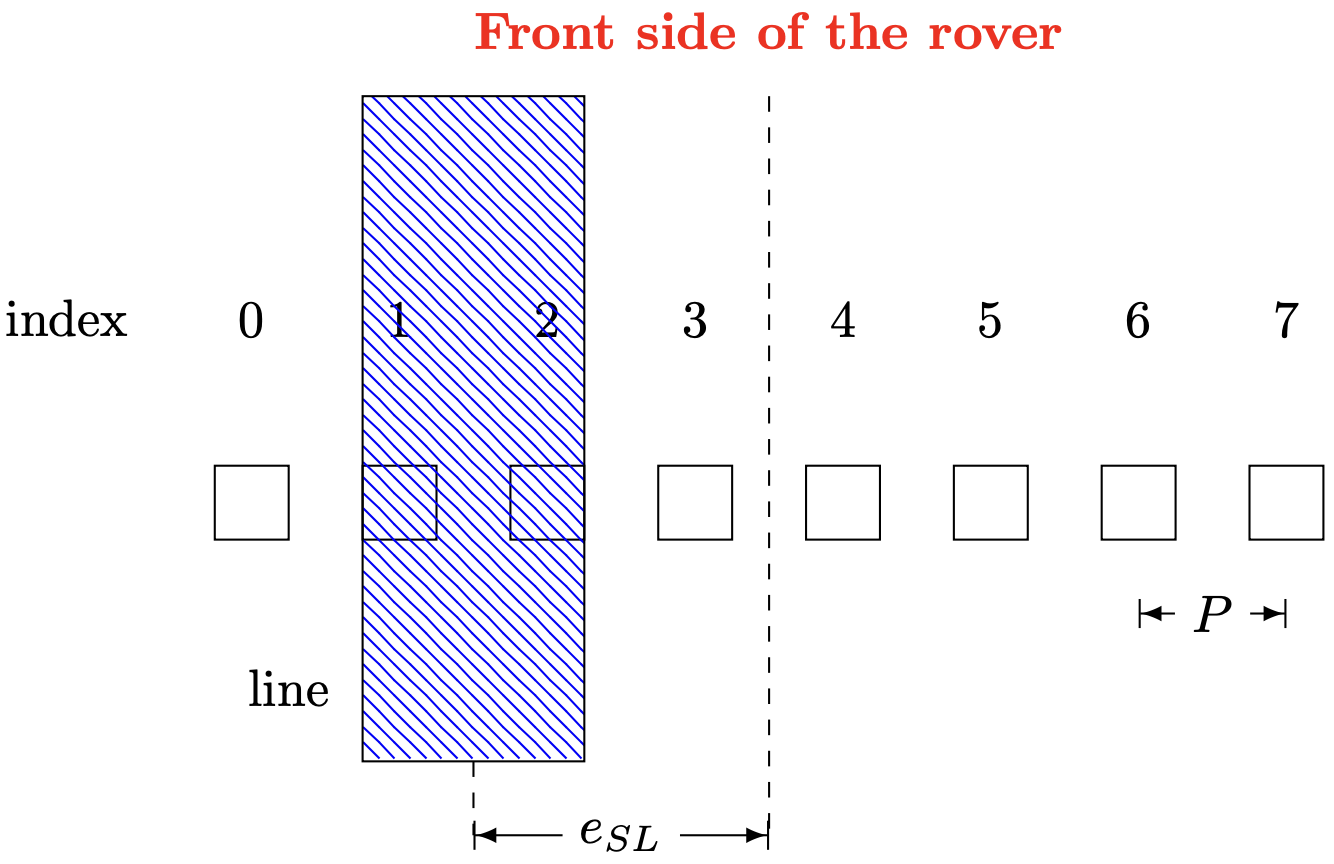
\includegraphics[width=0.7\textwidth]{lab4/figures/e_sl.png}
    \caption{Line tracking error}
    \label{fig:line_tracking_error}
\end{figure}

\subsubsection{Kinematic model}
In Figure~\ref{fig:kinematic_model} is shown the kinematic model of the robot used in this laboratory activity, whose mechanical parameters are reported in Table~\ref{tab: mech_param}.
\begin{table}[H]
    \centering
    \begin{tabular}{cc}
        \toprule
        \textbf{Parameter}  & \textbf{Value} \\
        \midrule
        Wheel distance ($D$) & 0.165 m \\
        Distance between the sensor and the vehicle's centre ($H$) & 0.085 m \\
        Wheel radius ($r$) & 0.034 m \\
        \bottomrule 
    \end{tabular}
    \caption{}
    \label{tab: mech_param}
\end{table}
The robot has two wheels that can be controlled independently, and in the following we assume a pure roll condition, i.e. the wheels do not slip on the ground.
The relations that connect the linear velocity of the wheels $V_l$ and $V_r$ with the angular velocities of the left and right wheels $\omega_l$ and $\omega_r$ are:
\begin{equation}
    V_r = r \cdot \omega_r, \quad V_l = r \cdot \omega_l
\end{equation}
where $r$ is the radius of the wheels.
The rotation of the robot is around the Instantaneous Center of Rotation (ICR), which is the point where the robot is not moving. The ICR is located at a distance $R$ from the center of the robot.
While, the distance between the two wheels is denoted as $D$. It holds that:
\begin{equation}
    V_r = \omega(R+D/2), \quad V_l = \omega(R-D/2)
\end{equation}
and by subtracking these two equations we obtain:
\begin{equation}
    \omega = \frac{V_r - V_l}{D}
\end{equation}

The angle $\psi$ between the global frame and the robot's frame is equal to the angle between the x-axis and the line connecting the ICR to the center of the robot, i.e. $\omega$.
Therefore, the yaw rate of the robot is equal to $\omega$, i.e.:
\begin{equation}
    \dot{\psi} = \frac{V_r - V_l}{D}
\end{equation}
Then, the linear velocity of the robot can be computed as the average of the linear velocities of the two wheels, i.e.:
\begin{equation}
    V = \frac{V_r + V_l}{2}
\end{equation}
And, finally, we derive the formulas which take into account both the longitudinal speed of the wheels and the yaw rate:
\begin{equation}
\begin{cases}
    V_r = V + \dot{\psi} \frac{D}{2} \\
    V_l = V - \dot{\psi} \frac{D}{2}
\end{cases}
\end{equation}
from which it immediately follows
\begin{equation}
\begin{cases}
    \label{eq:omega}
    \omega_r = \frac{V + \dot{\psi} \frac{D}{2}}{r} \\
    \omega_l = \frac{V - \dot{\psi} \frac{D}{2}}{r}
\end{cases}
\end{equation}
\begin{figure} [H]
    \centering
    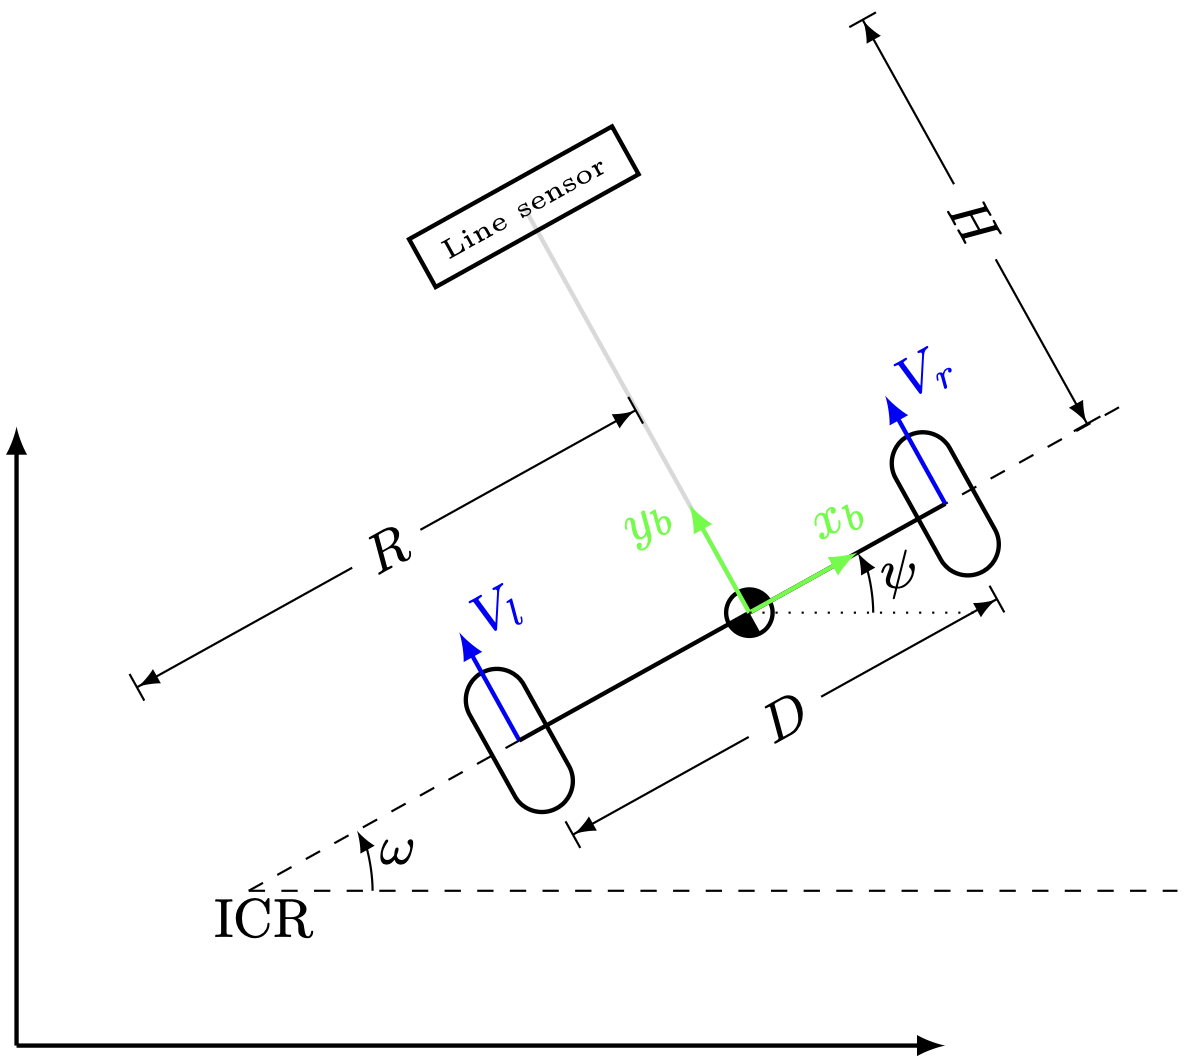
\includegraphics[width=0.6\textwidth]{lab4/figures/kinematic_model.png}
    \caption{Kinematic model}
    \label{fig:kinematic_model}
\end{figure}

\subsubsection{Yaw error}
At this point, we need to define the yaw error, which is the difference between the desired yaw angle ($\psi_{ref}$) and the actual yaw angle ($\psi$) of the robot. The yaw error can be expressed as:
\begin{equation}
    \psi_{err} = \psi_{ref} - \psi
\end{equation}

The relationship between the yaw error and the line tracking error can be expressed as follows:
\begin{equation}
    \label{eq:psi_err}
    \psi_{err} = \arctan\left(\frac{e_{SL}}{H}\right) \approx \frac{e_{SL}}{H}
\end{equation}
Where the last equation exploits the small angle approximation, which is valid for small values of $e_{SL}$.